\apendice{Especificación de Diseño}
\label{apendice:diseno}

\section{Introducción}
La fase de diseño permite planificar un proyecto para su correcta implementación, desarrollo y evolución. En este anexo se exponen los diferentes diseños que se han llevado a cabo para obtener una solución robusta y escalable a los problemas planteados. Se detallará el diseño de los datos que maneja el sistema, el diseño arquitectónico de alto nivel, y el diseño procedimental que describe el flujo de trabajo del pipeline.

\section{Diseño de Datos}
\label{sec:diseno_datos}
El diseño de datos se centra en la estructura y el formato de la información que fluye a través del sistema. Aunque el dato principal es el vídeo, su tratamiento y los metadatos asociados son clave.

\subsection{Objeto de Datos Principal: Vídeo de Sesión}
El dato principal que se procesa es el archivo de vídeo generado por Jibri. Este es un fichero en formato \textbf{MP4}, que contiene un \textit{stream} de vídeo codificado (normalmente con el \textit{códec} H.264) y un \textit{stream} de audio.

\subsection{Formato de Salida del Procesamiento}
Una de las tareas de la fase final del proyecto es definir el formato de salida que generará el \textit{script} de Spark. Se ha establecido que el resultado será un nuevo fichero de vídeo también en formato MP4. Para una futura evolución del proyecto donde se extraigan características específicas, se podría definir un formato de datos estructurado (como JSON o Avro) que contenga metadatos como:
\begin{itemize}
    \item \texttt{id\_sesion}: Identificador único de la sesión grabada.
    \item \texttt{timestamp}: Marca de tiempo del procesamiento.
    \item \texttt{algoritmo\_aplicado}: Nombre de la transformación realizada (ej. "inversion-color").
    \item \texttt{ruta\_video\_procesado}: Ruta al fichero de vídeo resultante.
    \item \texttt{métricas}: Un objeto que podría contener métricas de análisis (ej. número de objetos detectados, nivel de movimiento, etc.).
\end{itemize}

\section{Diseño Arquitectónico}
\label{sec:diseno_arquitectonico}
El diseño arquitectónico define la estructura de alto nivel del sistema, sus componentes principales y las interacciones entre ellos.

\subsection{Diagrama de Arquitectura General del Sistema}
La arquitectura general se ha diseñado como un sistema distribuido basado en micro-servicios, donde cada componente tiene una responsabilidad única. La Figura \ref{fig:arquitectura_general} ofrece una visión completa de la solución, desde la captura de vídeo hasta el procesamiento final.

\begin{figure}[H]
    \centering
    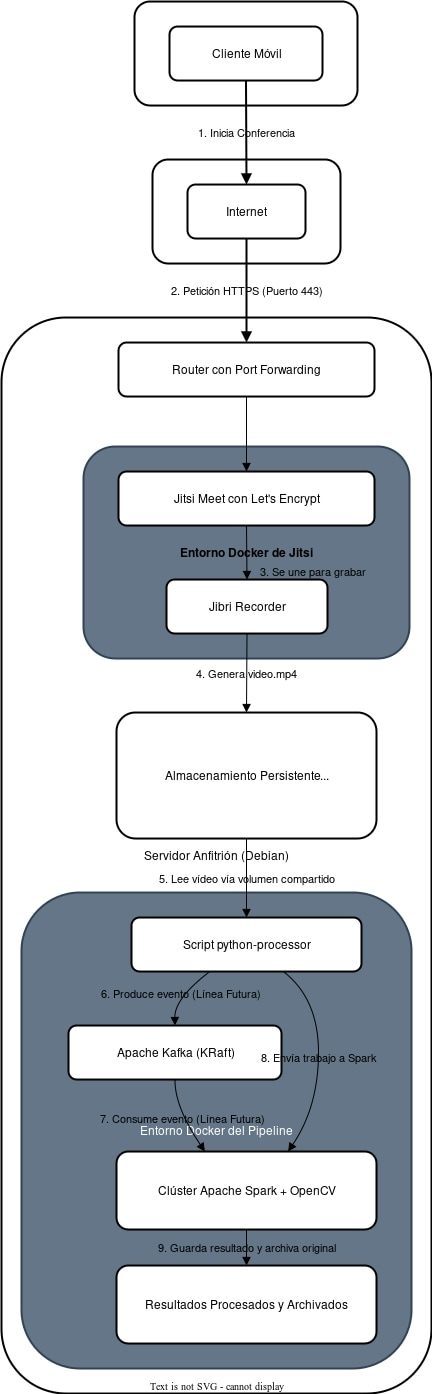
\includegraphics[height=\textheight]{img/arquitectura-general.jpg}
    \caption{Diagrama de la arquitectura general del sistema.}
    \label{fig:arquitectura_general}
\end{figure}

Como se puede observar, el sistema se divide en tres grandes bloques: el subsistema de captura de vídeo (basado en Jitsi), el pipeline de datos (orquestado con Docker Compose y centrado en Kafka y Spark), y el almacenamiento persistente.

\subsection{Diagrama de la Arquitectura de Red para Jitsi}
El despliegue de Jitsi para que fuera accesible desde el exterior de forma segura fue uno de los principales desafíos técnicos. La solución final, representada en la Figura \ref{fig:arquitectura_red}, se basa en una configuración de red que incluye un servicio de DNS dinámico, redirección de puertos y la generación de certificados SSL/TLS con Let's Encrypt.

\begin{figure}[H]
    \centering
    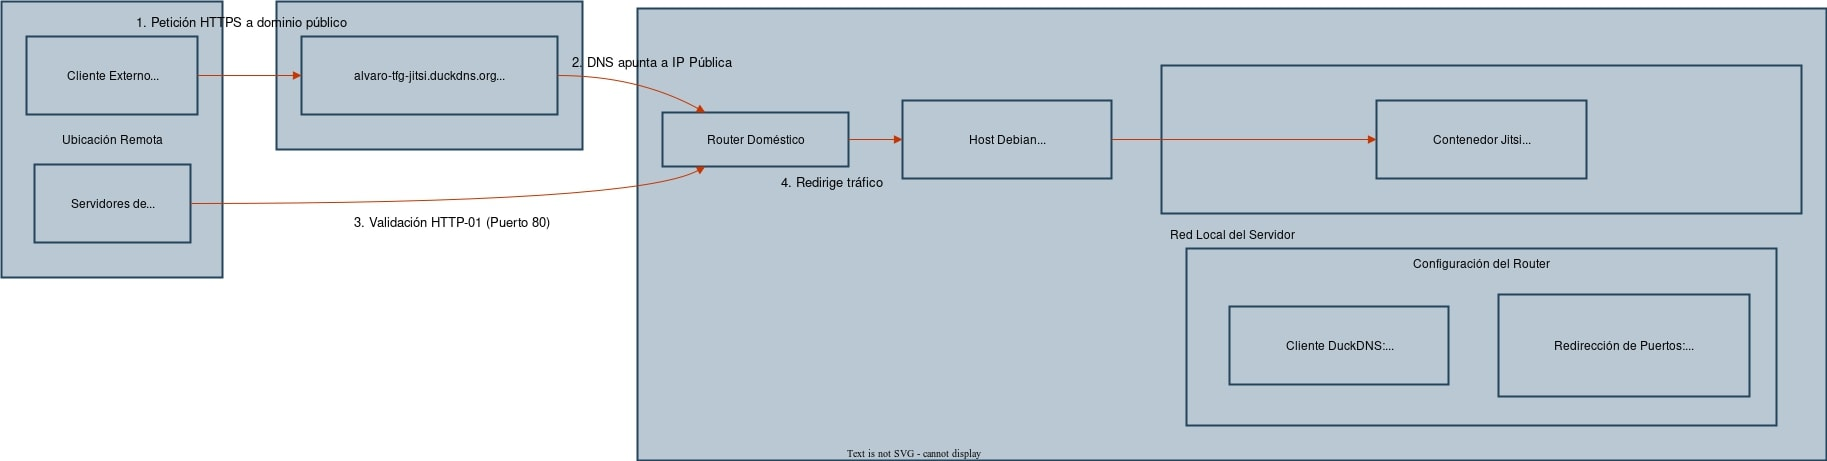
\includegraphics[width=1\textwidth]{img/ArquitecturadeRedparaelDesplieguedeJitsi.jpg}
    \caption{Arquitectura de red para el despliegue seguro de Jitsi.}
    \label{fig:arquitectura_red}
\end{figure}

\section{Diseño Procedimental}
\label{sec:diseno_procedimental}
El diseño procedimental describe la secuencia de pasos y el flujo de control del sistema.

\subsection{Flujo de Datos del Pipeline de Procesamiento}
El núcleo de la lógica de negocio reside en el pipeline implementado dentro del directorio \texttt{/src}. El flujo de datos (ver Figura \ref{fig:flujo_pipeline}) describe la interacción entre el \textit{script} de Python, Kafka y Spark para procesar los vídeos de forma automatizada.

\begin{figure}[H]
    \centering
    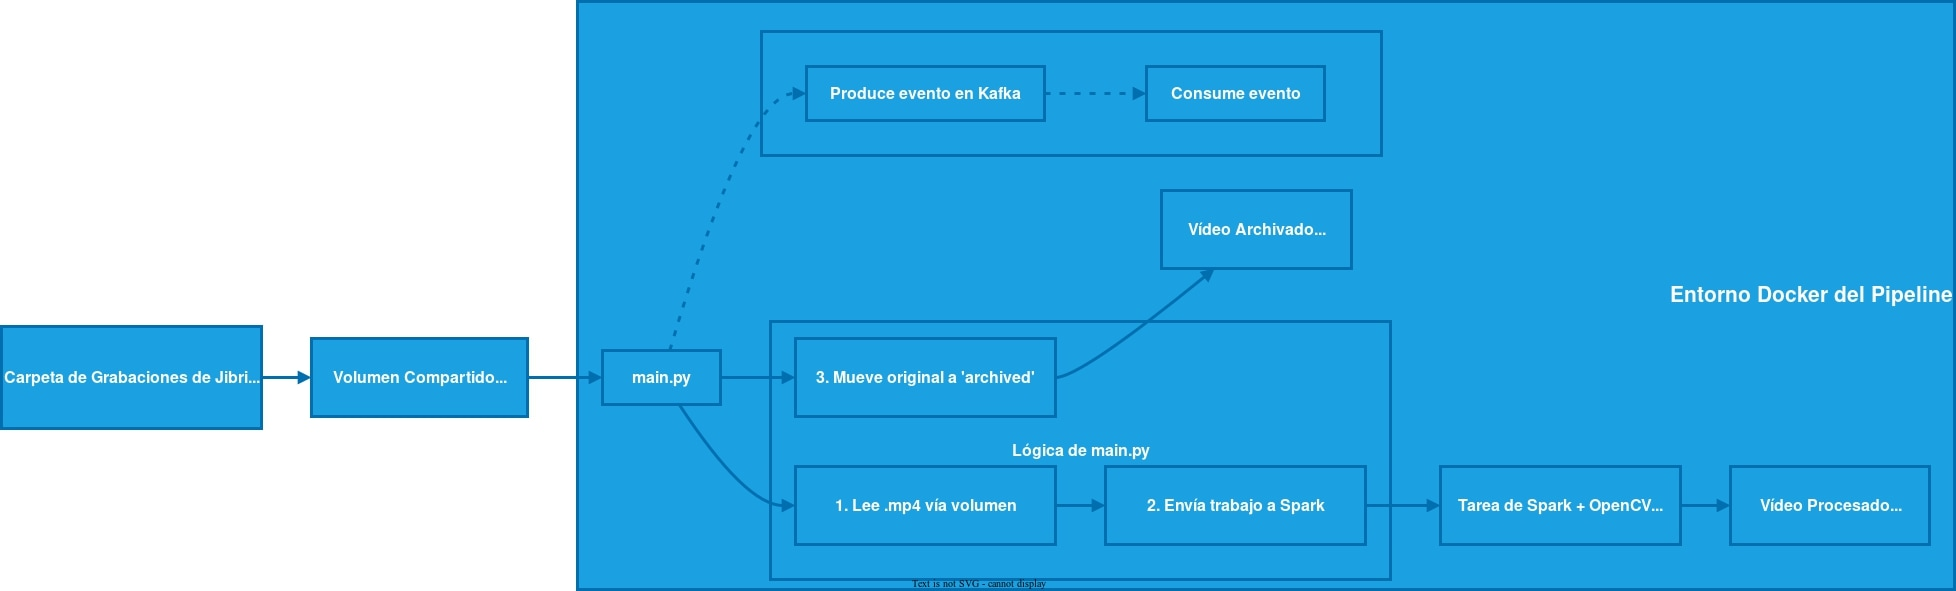
\includegraphics[width=\textwidth]{img/FlujodeDatosdelPipelinedeProcesamiento.jpg}
    \caption{Diagrama de flujo de datos del pipeline de procesamiento.}
    \label{fig:flujo_pipeline}
\end{figure}

El proceso comienza cuando el \textit{script} principal detecta un nuevo archivo MP4. Este archivo es enviado como un mensaje a Kafka. Un consumidor de Spark recibe el mensaje, ejecuta la lógica de procesamiento y guarda el resultado, archivando finalmente el vídeo original.

\subsection{Funcionamiento Interno de la Grabación de Jibri}
Para comprender cómo se genera la fuente de datos, es útil visualizar el funcionamiento interno de Jibri (Figura \ref{fig:flujo_jibri}). Jibri lanza una instancia de un navegador en modo \textit{headless} que se une a la conferencia, renderiza la vista compuesta y utiliza FFmpeg para capturar esta salida y codificarla en un archivo MP4.

\begin{figure}[H]
    \centering
    \includegraphics[width=0.8\textwidth]{img/ProcesoInternodeGrabacióndeJibri..jpg}
    \caption{Diagrama conceptual del proceso de grabación de Jibri.}
    \label{fig:flujo_jibri}
\end{figure}

\subsection{Casos de Uso del Sistema}
Finalmente, el diagrama de casos de uso (Figura \ref{fig:casos_uso}) muestra la interacción de los diferentes actores (Técnico, Usuario, Terapeuta) con las funcionalidades principales del sistema.

\begin{figure}[H]
    \centering
    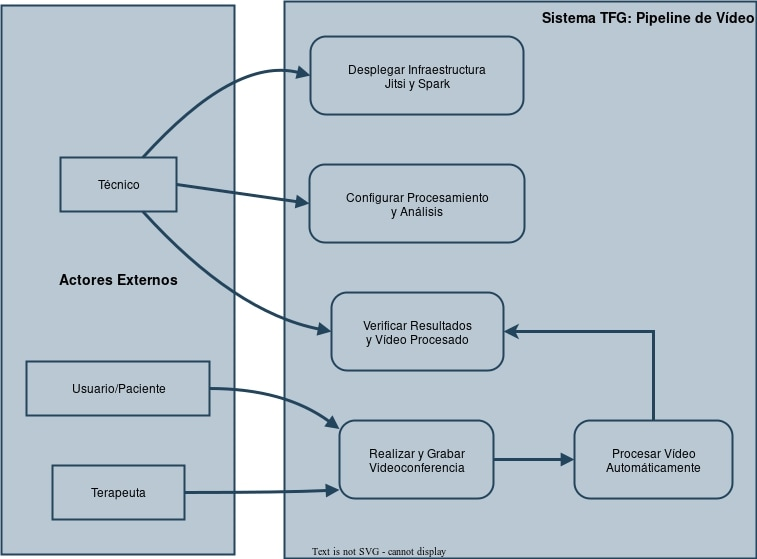
\includegraphics[width=0.7\textwidth]{img/Diagramacasodeuso.jpg}
    \caption{Diagrama de los principales casos de uso del sistema.}
    \label{fig:casos_uso}
\end{figure}

\subsection{Flujo Detallado de Transformación en Spark}
Para comprender en profundidad cómo se procesan los datos una vez que llegan al consumidor de Spark, la Figura \ref{fig:flujo_transformacion_spark} detalla el flujo de transformación de paquetes que se ejecuta dentro del script de PySpark.

\begin{figure}[H]
    \centering
    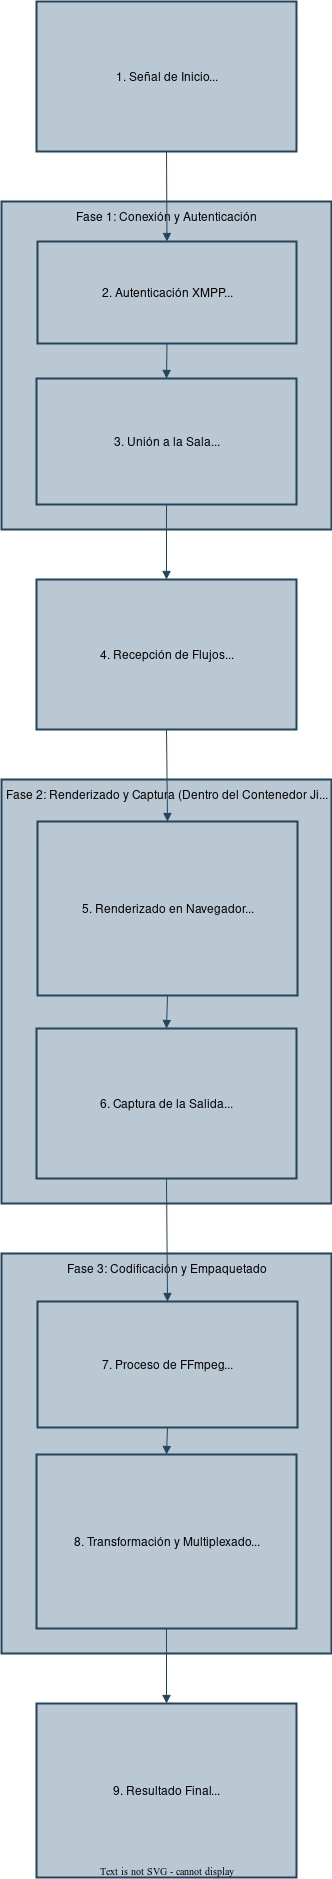
\includegraphics[height=\textheight]{img/FlujoDetalladodeTransformaciondePaquetes.jpg}
    \caption{Diagrama de flujo detallado del procesamiento de vídeo en Spark.}
    \label{fig:flujo_transformacion_spark}
\end{figure}

El proceso procedimental es el siguiente:
\begin{enumerate}
    \item El consumidor Spark recibe un mensaje desde el \textit{topic} de Kafka. Este mensaje contiene los datos o la referencia al vídeo a procesar.
    \item Los datos son pasados a una función de procesamiento definida por el usuario.
    \item Dentro de esta función, se utiliza la librería OpenCV para abrir el fichero de vídeo y comenzar a leerlo fotograma a fotograma.
    \item Se itera sobre cada \textit{frame}: se aplica la transformación de vídeo correspondiente (en la prueba de concepto, una inversión de color) y el \textit{frame} modificado se escribe en un nuevo fichero de vídeo de salida.
    \item Una vez procesados todos los \textit{frames}, se cierra el flujo de escritura, finalizando la creación del vídeo procesado.
\end{enumerate}
Este diseño modular permite que la lógica de transformación (paso 4) pueda ser fácilmente modificada o extendida en el futuro para aplicar análisis más complejos.

Para poder ver correctamente los diagramas debido a su tamaño se recomienda descargarlos de la documentación.